\begin{figure*}[!t]
	\begin{center}
		\subfigure[No Failure]
		{
			\label{fig:sc_no_fail}
			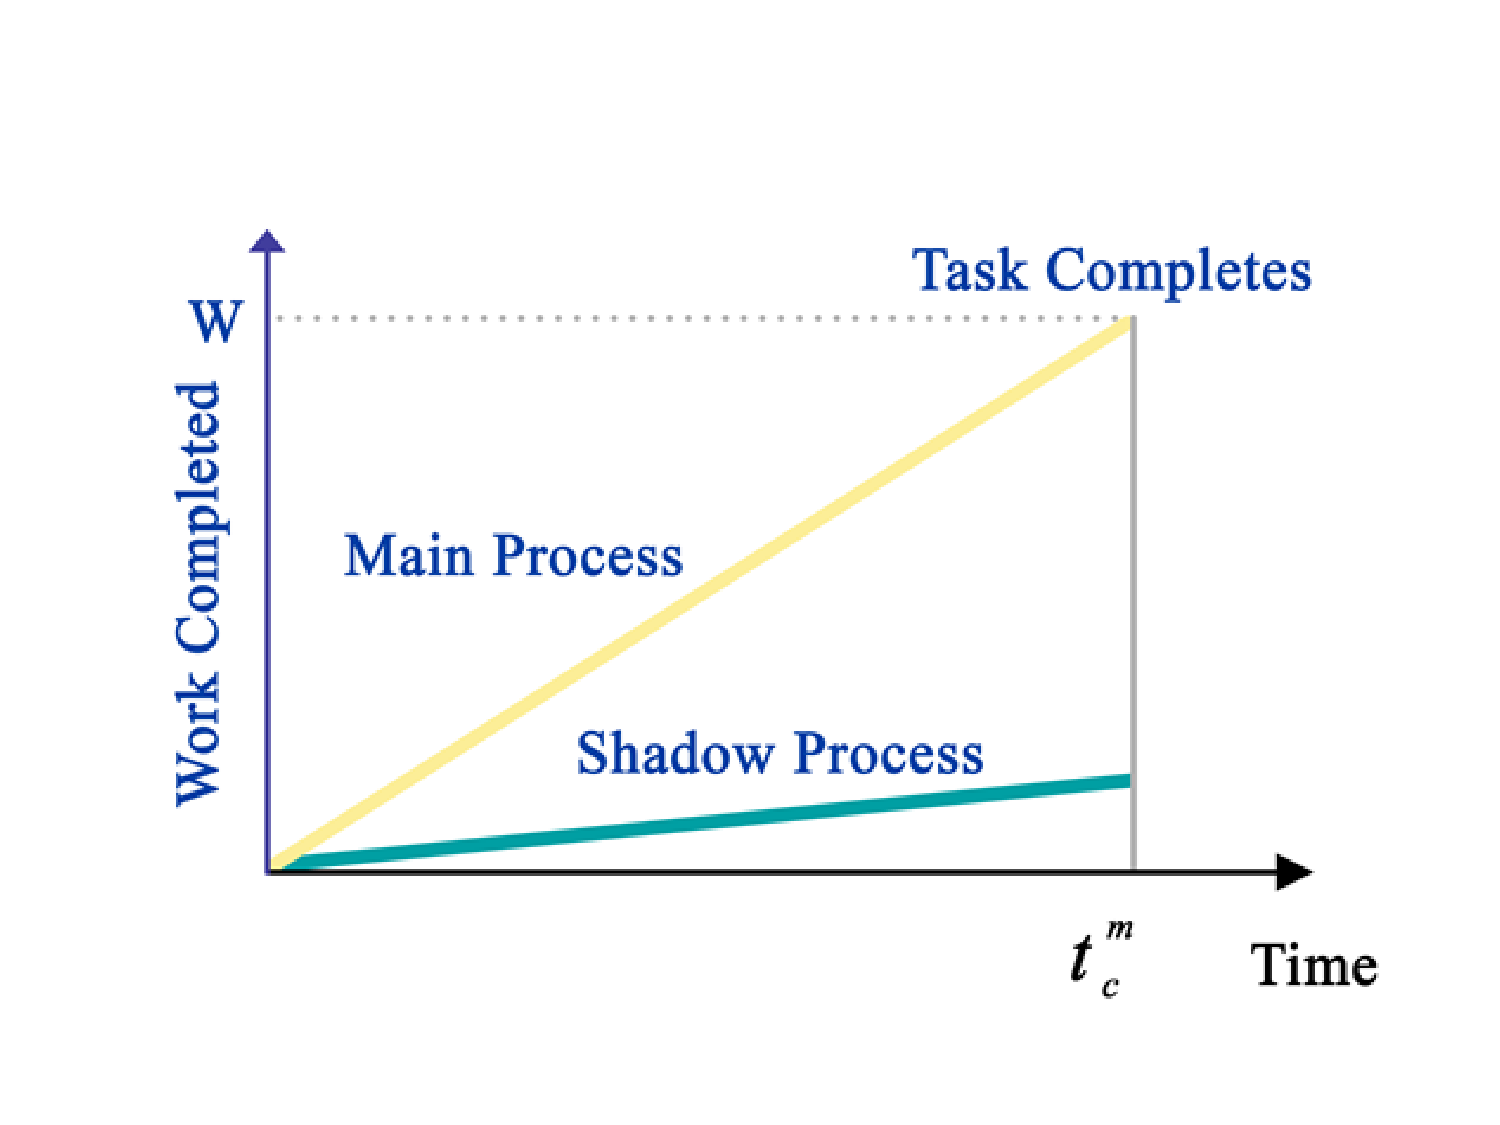
\includegraphics[width=0.32\textwidth]{diagrams/example1.pdf}
		}
		\subfigure[Shadow Process Failure]
		{
			\label{fig:sc_shadow_fail}
			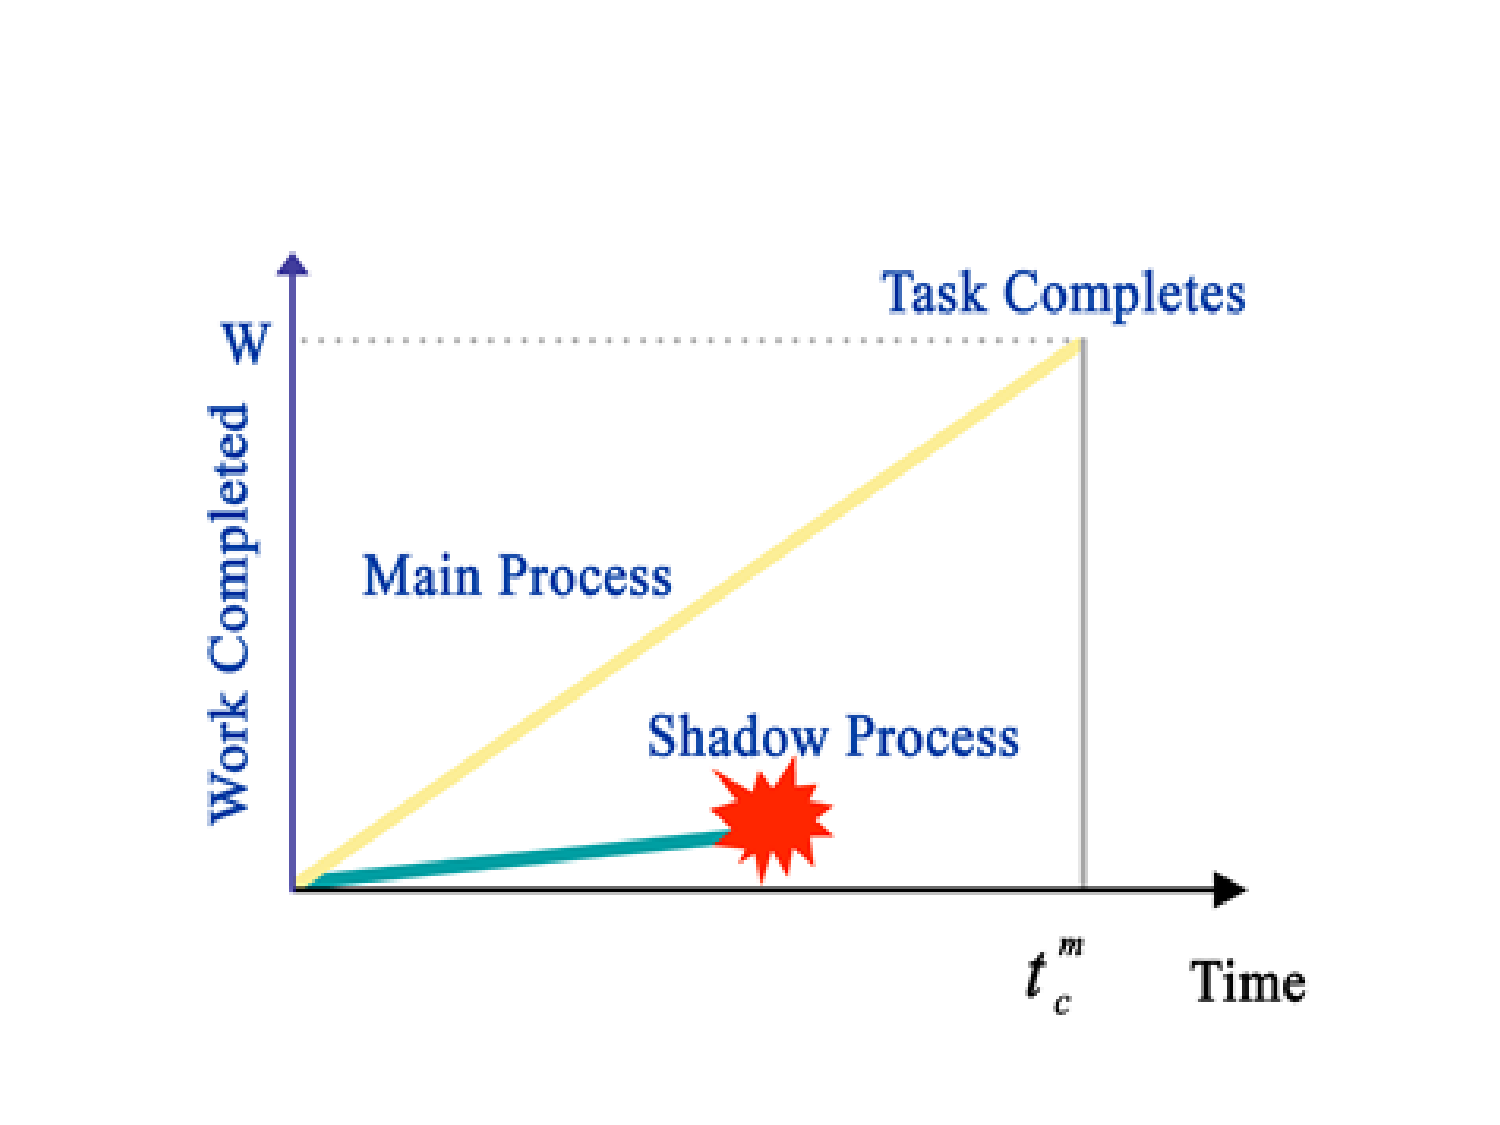
\includegraphics[width=0.29\textwidth]{diagrams/example3.pdf}
		}
		\subfigure[Main Process Failure]
		{
			\label{fig:sc_main_fail}
			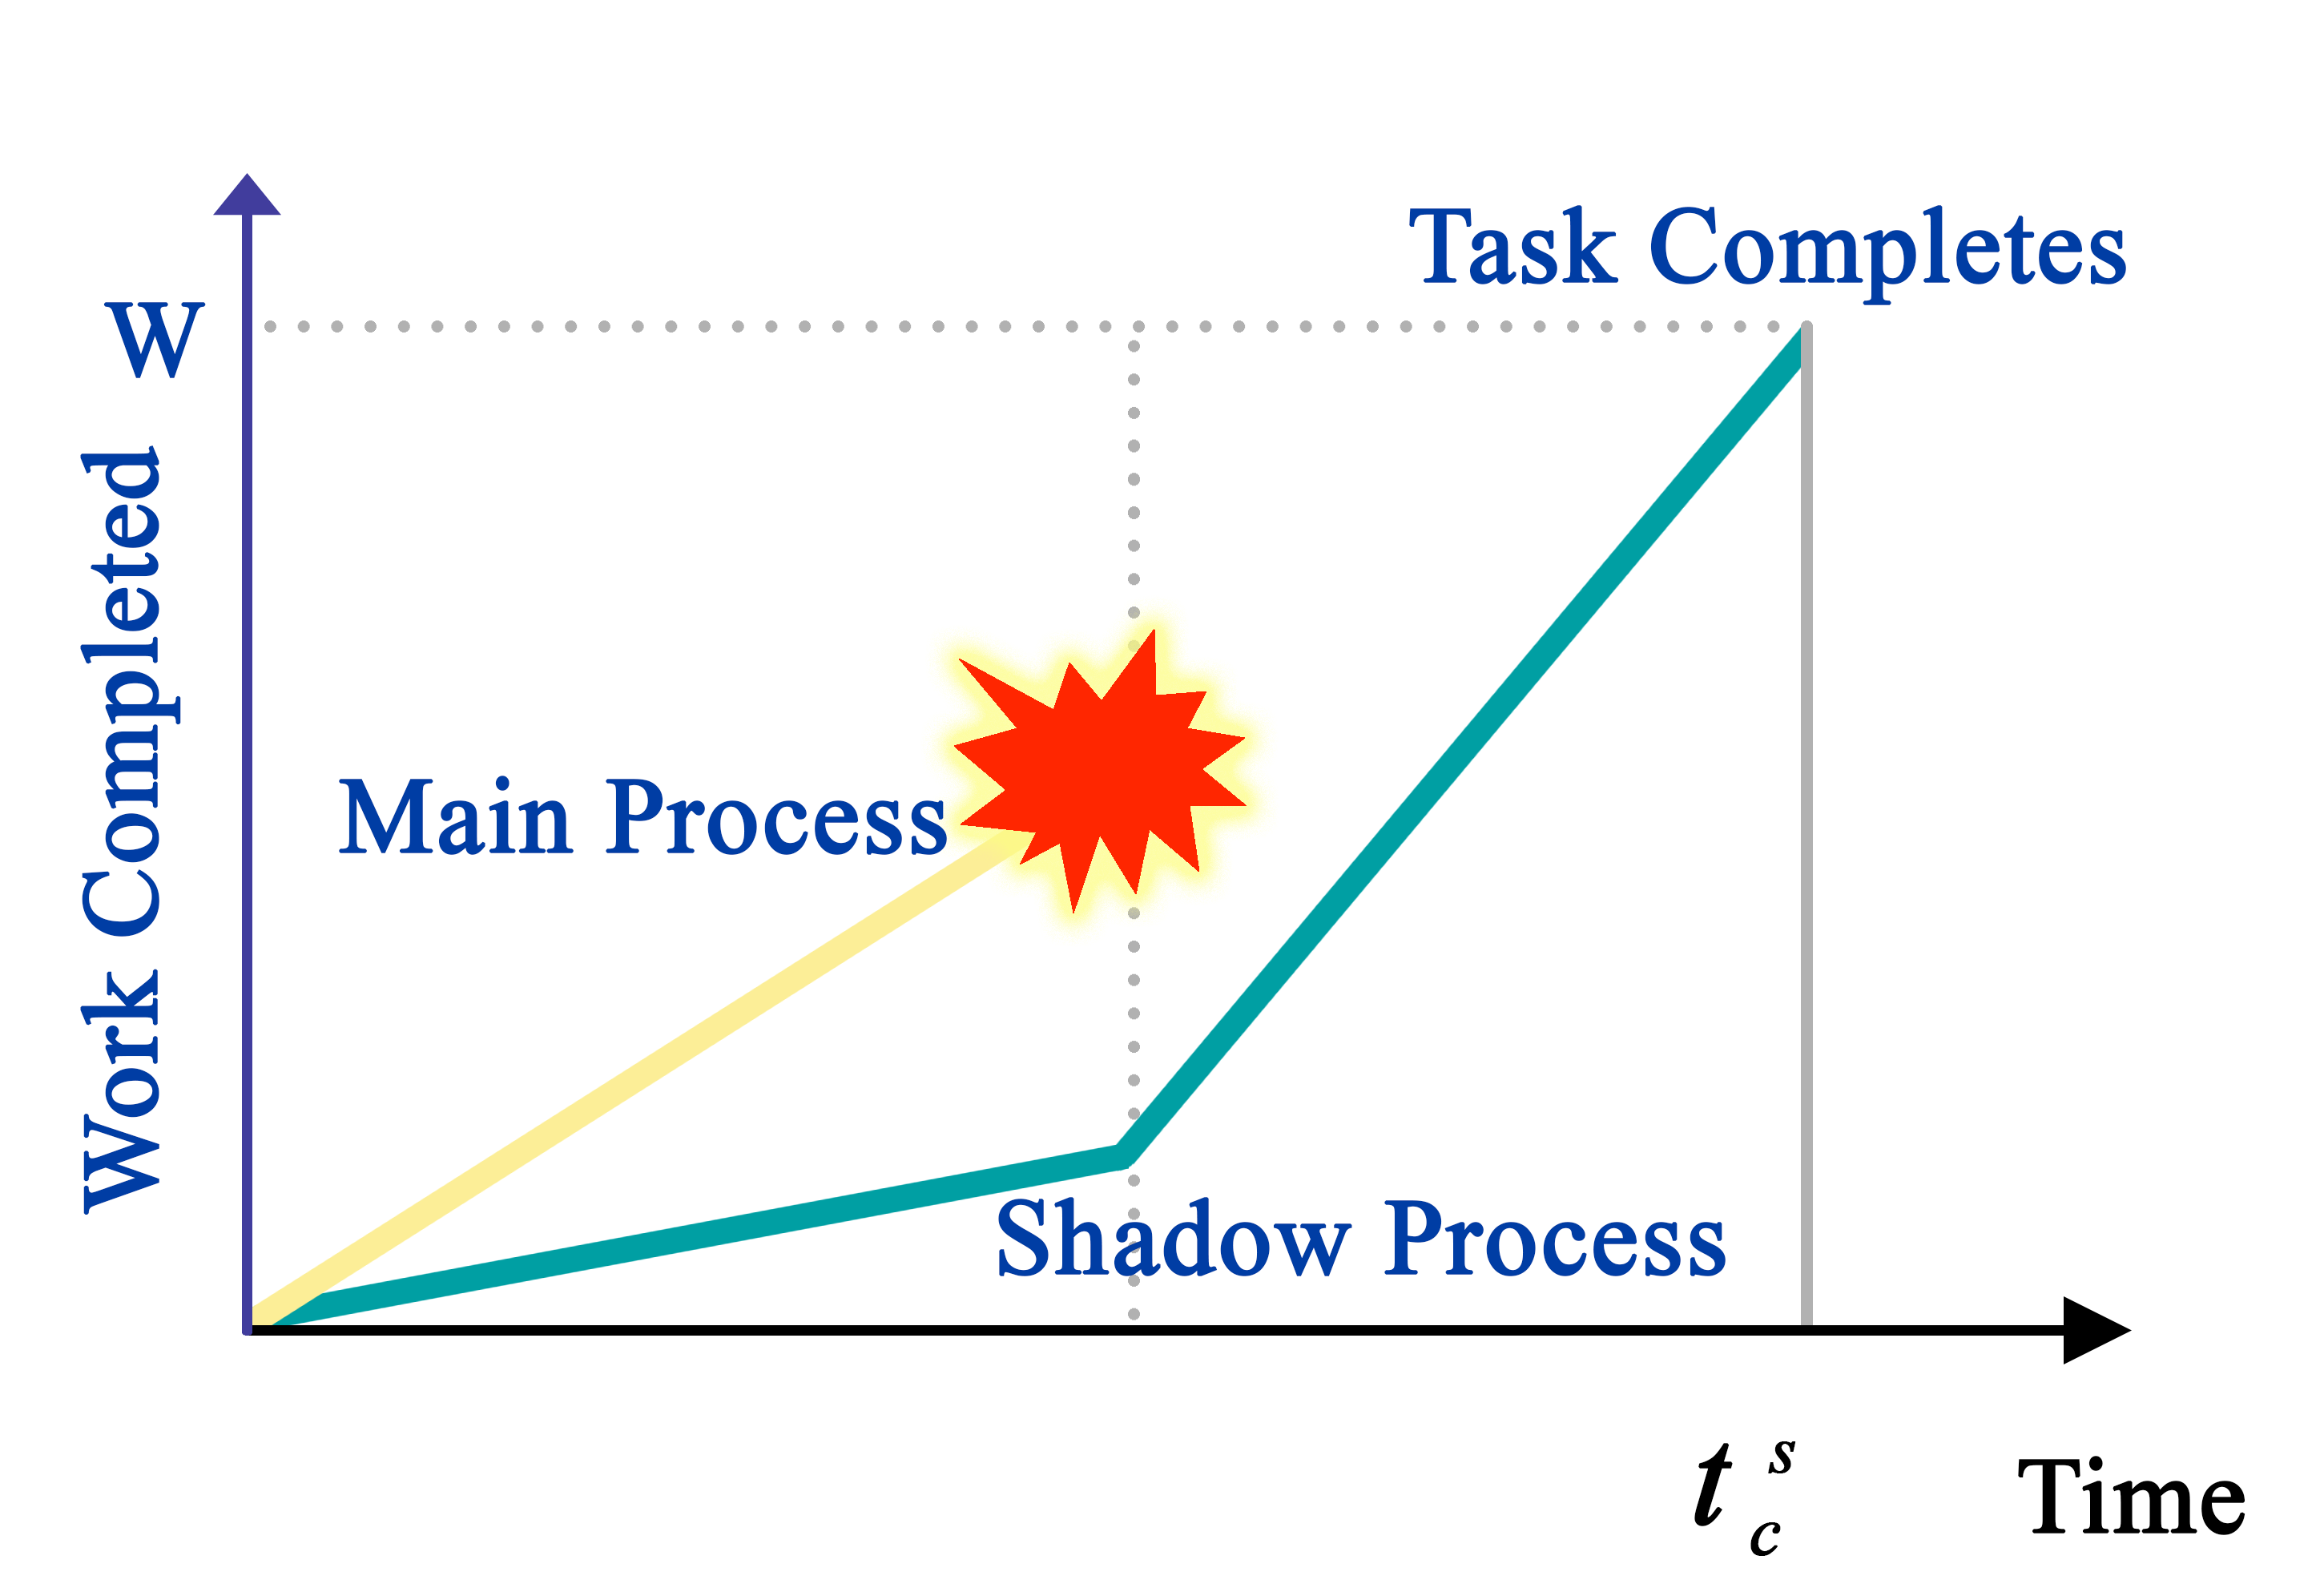
\includegraphics[width=0.33\textwidth]{diagrams/example2.png}
		}
	\end{center}
	\caption{Shadow replication for a single task and single replica}
	\label{fig:sc_overview}
\end{figure*}

\noindent 
The basic tenet of Shadow Replication is to associate with each
main process a suite of ``shadows'' whose size depends on the
``criticality'' of the application and its performance requirements,
as defined by the SLA. 
%To overcome potential failures, the shadows
%execute on separate computing nodes, concurrently with but at slower
%speeds than, the main process.

%The successful completion of the main
%process results in the immediate termination of all shadow
%processes. If the main process fails, the primary shadow process takes
%over the role of the main process and resumes computation, possibly at
%an increased speed, in order to complete the task at a targeted
%response time.


Formally, we define the Shadow Replication fault-tolerance model as follows:
\begin{itemize}
\item A main process, $P_m(W,\text{ }\sigma_m)$, whose responsibility is to executes a task of size $W$ at a speed of $\sigma_m$;
\item A suite of shadow processes, $P_{s}(W,\text{ }\sigma_b^s, \text{ }\sigma_a^s)$ ($1 \le s \le \cal S)$, where $\cal S$ is the size of the suite. 
The shadows execute on separate computing nodes. Each shadow process is associated with two execution speeds. All shadows start execution simultaneously with the main process at speed $\sigma_b^s$ ($1 \le s \le \cal S$). Upon failure of the main process, all shadows switch their executions to $\sigma_a^s$, with one shadow being designated as the new main process. This process continues until completion of the task.
\end{itemize}
%All shadows execute simultaneously with the main process at speed $\sigma_a^s$

To illustrate the behavior of Shadow Replication, we limit the number of shadows to a single process and consider the scenarios depicted in Figure \ref{fig:sc_overview}, assuming a single process failure. Figure \ref{fig:sc_no_fail} represents the case when neither the main nor the shadow fails. The main process, executing
at a higher speed, completes the task at time $t_c^m$. At this time, the shadow process, progressing at a lower speed, stops execution immediately. Figure \ref{fig:sc_shadow_fail} represents the case when the shadow fails. This failure, however, has no impact on the progress of the main process, which still completes the task at $t_c^m$. Figure \ref{fig:sc_main_fail} depicts the case when the main process fails while the shadow is in progress. After detecting the failure of the main process, the shadow begins execution at a higher speed, completing the task at time $t_c^s$. When possible, the shadow execution speed upon failure must be set so that $t_c^s$ does not exceed $t_c^m$. Given that the failure rate of an individual node is much lower than
the aggregate system failure, it is very likely that the main process
will always complete its execution successfully, thereby achieving fault tolerance at a significantly reduced cost of energy consumed by the shadow. %saving a lot of energy for its associated shadow processes. 

%In summary, shadow replication has the following characteristics:
%The proposed shadow replication model has several properties:
%\begin{itemize}
%\item The main process is associated with only one execution speed, $\sigma_m$, %which depends on the size of the task and the SLA requirement.
%\item The shadow processes execute with two different speeds, which are failure %dependent and when possible should be computed to meet the SLA requirement as %closely as possible. 
%\item The completion of the main process results in the immediate termination of %all shadow processes. Given that the failure rate of an individual node is much %lower than the aggregate system failure, it is very likely that the main process %completes successfully, saving a significant amount of energy, while achieving %high level of fault tolerance.
%\end{itemize}


A closer look at the model reveals that shadow
replication is a generalization of traditional fault tolerance
techniques, namely re-execution and traditional replication. If the
SLA specification allows for flexible completion time, shadow
replication would take advantage of the delay laxity to trade time
redundancy for energy savings. It is clear, therefore, that for a
large response time, Shadow Replication converges to re-execution, as
the shadow remains idle during the execution of the main process and
only starts execution upon failure. If the target response time is
stringent, however, Shadow Replication converges to pure replication,
as the shadow must execute simultaneously with the main at the same
speed. The flexibility of the Shadow Replication model provides the
basis for the design of a fault tolerance strategy that strikes a
balance between task completion time and energy saving, thereby
maximizing profit.

As stated previously, the large amount of data being
processed requires the use of thousands, if not millions, of tasks during each phase. As
the number tasks increases, the likelihood of failure during an
individual phase will also increase. Fault tolerance is critical at
the phase-level because the delay of one task results in a delay of
the entire phase. Hence, techniques such as shadow replication would
be applied to each phase independently. Due to the independence
between phases, we focus on the fault-tolerance issues related to one computing phase 
of a cloud computing job.


The feasibility of shadow replication, as an energy-aware, fault-tolerant model for cloud computing, requires
a methodology to determine the speeds, both before and after a failure occurs, 
at which the main process and its associated shadow must execute to meet the performance 
and resiliency SLA requirements of the supported application.  
In the following section, we describe a profit-based optimization framework to compute the optimal
speeds of the shadow replication processes. In this framework, it is assumed that
failures can be detected.  While this is the case in many computing
environments, there are cases where failure detection may not be
possible. To address this limitation, we propose, "streched replication, a sub-optimal shadow
replication scheme, whereby both the main process and its associated shadow
execute independently at stretched execution speeds to meet the expected
response time and achieve the expected level of failure tolerance. Streched replication does not additional mechanisms for main process failure
detection. Finally, the expected energy consumption of "reexecution", a commonly used fault-tolerance model
in cloud computing, is described. Both models are used in the fault-tolerance comparative analysis carried out in this paper.
 
